\section{Iteración 1}
\label{sec:iteracion_1}

Para la primera iteración se implementaran las historias de usuario que tengan más relevancia dentro de la lógica de negocios para el cliente, generalmente son las que tienen mayor impacto en el sistema a desarrollar.


\subsection{Iteration Planning Meeting}
\label{sub:Iteration Planning Meeting}


Tomando en cuenta que el equipo de desarrollo está compuesto solo por mi persona, para el desarrollo del presente proyecto de grado la fase de Exploración y Planeación se procedió a realizarlas en la misma fase.

  \subsubsection{Exploración y Planeación}
  \label{subs:Exploración y Planeación}

Para la primera iteración se llevó a cabo una reunión para determinar las historias de usuario que se implementaran, y de acuerdo del impacto en el producto se determinó que las historias de usuario 2 y 3 serán las primeras en implementarse. \\

Posteriormente como tarea del desarrollador se procede a dividir las historias de usuario en Tareas de Ingeniería, en la tabla se determinaron las Tareas pertenecientes a la historia de usuario 2, dentro lo que es la planeación se debe repartir las tareas entre los desarrolladores, pero ya que el equipo de desarrollo se traduce a mi persona, todas las tareas recaen sobre mi responsabilidad, como parte de la planeación es necesario estimar las tareas, para lo cual se presenta la tabla \ref{tab:us02_tasks}. \\


  \subsection{Tareas del US02}
  \label{sub:us02_tasks}

    \begin{table}[H]
  \begin{center}
    \begin{tabularx}{\textwidth}{ c  X  C{2.3cm} }
      \toprule
        \textbf{Código} &
        \multicolumn{1}{c}{\textbf{Tarea}} &
        \textbf{Estimación [dias]}\\

      \midrule
        RF001
        &
        Crear un archivo shapefile con información inicial de lugares principales dentro el campus de la UMSS.
        &
        1 \\

      \addlinespace
        RF002
        &
        Crear una base de datos que pueda manejar información geoespacial.
        &
        1 \\

      \addlinespace
        RF003
        &
        Popular la base de datos creada en RF002 con la información de RF001.
        &
        0.5 \\

      \addlinespace
        RF004
        &
        El usuario puede ver una lista con los lugares creados.
        &
        2 \\

      \addlinespace
        RF005
        &
        El usuario deberá poder ingresar el nombre de un lugar para filtrar los lugares existentes.
        &
        0.5 \\

      \addlinespace
        RF006
        &
        El usuario deberá poder ver la información de un lugar al hacer tap sobre el nombre del lugar en la lista.
        &
        1 \\

      \addlinespace
        TS001
        &
        Crear pruebas de funcionalidad del US02.
        &
        1 \\

      \addlinespace
      \midrule
        & \multicolumn{1}{R{7cm}}{\textbf{Total: }}
        & 7 \\

      \bottomrule
    \end{tabularx}
    \caption{Tareas de la US02}
    \label{tab:us02_tasks}
  \end{center}
\end{table}


  \subsection{Tareas del US03}
  \label{sub:us03_tasks}

    
\begin{table}[H]
  \begin{center}
    \begin{tabularx}{\textwidth}{ c  X  C{2.3cm} }
      \toprule
        \textbf{Código} &
        \multicolumn{1}{c}{\textbf{Tarea}} &
        \textbf{Estimación [dias]}\\

      \midrule
        RF007
        &
        El usuario puede ver la descripción del lugar.
        &
        0.5 \\

      \addlinespace
        RF008
        &
        El usuario puede ver el teléfono del lugar.
        &
        0.5 \\

      \addlinespace
        RF009
        &
        El usuario puede ver en qué piso se encuentra el lugar.
        &
        0.5 \\

      \addlinespace
        RF010
        &
        El usuario puede ver una imagen del lugar.
        &
        1 \\

      \addlinespace
        TS002
        &
        Crear pruebas de funcionalidad del US03.
        &
        0.5 \\

      \addlinespace
      \midrule
        & \multicolumn{1}{R{7cm}}{\textbf{Total: }}
        & 3 \\

      \bottomrule
    \end{tabularx}
    \caption{Tareas de la US03}
    \label{tab:us03_tasks}
  \end{center}
\end{table}



  \subsection{Calendario de Entregas}
  \label{subs:schedule_1}

    % \begin{table}[!ht]
%
% \end{table}
\begin{table}[H]

  \begin{center}

\begin{ganttchart}[
  canvas/.append style={fill=none, draw=black!5, line width=.75pt},
  hgrid style/.style={draw=black!5, line width=.75pt},
  vgrid={*1{draw=black!5, line width=.75pt}},
  %today=0,
  % today label=Semana 3,
  today rule/.style={
    draw=black!64,
    dash pattern=on 3.5pt off 4.5pt,
    line width=1.5pt
  },
  today label font=\small\bfseries,
  title/.style={draw=none, fill=none},
  title label font=\bfseries\footnotesize,
  title label node/.append style={below=7pt},
  include title in canvas=false,
  bar label font=\mdseries\small\color{black!70},
  bar label node/.append style={left=2cm},
  bar/.append style={draw=none, fill=black!63},
  bar incomplete/.append style={fill=barblue},
  bar progress label font=\mdseries\footnotesize\color{black!70},
  group incomplete/.append style={fill=groupblue},
    group left shift=0,
    group right shift=0,
    group height=.5,
    group peaks tip position=0,
    group label node/.append style={left=.6cm},
    group progress label font=\bfseries\small,
    link/.style={-latex, line width=1.5pt, linkred},
    link label font=\scriptsize\bfseries,
    link label node/.append style={below left=-2pt and 0pt},
  ]{1}{12}
  \gantttitle{Calendario de Entregasde de la Iteración 1}{7} \\[grid]
  \gantttitle{Semana 1}{7}
  \gantttitle{Semana 2}{7} \\
  % \gantttitle{Noviembre}{4} \\
  \gantttitle[title label node/.append style={below left=7pt and -3pt}]{D\'ia:\quad1}{1}
  \gantttitlelist{2,...,14}{1} \\
  % \ganttgroup[progress=0]{Historias de Usuario}{1}{8} \\
  \ganttbar[
    progress=0,
    name=bar1
  ]{\textbf{User Story 01}}{1}{9} \\
  \ganttbar[
    progress=0,
    name=bar2
  ]{\textbf{User Story 02}}{10}{12} \\
  % \ganttbar[
  %   progress=0,
  %   name=bar3
  % ]{\textbf{Iteración 3}}{5}{6} \\
  % \ganttbar[
  %   progress=0,
  %   name=bar4
  % ]{\textbf{Iteración 4}}{7}{8} \\
  % \ganttbar[
  %   progress=100,
  %   name=bar5
  % ]{\textbf{Actividad 5}}{5}{7} \\
  % \ganttbar[
  %   progress=80,
  % ]{\textbf{Actividad 6}}{8}{8} \\
  % \ganttbar[
  %   progress=49,
  % ]{\textbf{Actividad 7}}{9}{11} \\
  % \ganttmilestone{Hito 1}{11}{11}  \\
  % \ganttmilestone{Hito 2}{12}{12} \\
  %

  % \ganttmilestone{Q6 report}{24}{24} \\
  % \ganttmilestone{M1: Project finished}{8}{8}

  \ganttlink[link type=f-s]{bar1}{bar2}
  % \ganttlink[link type=f-s]{bar2}{bar3}
  % \ganttlink[link type=f-s]{bar3}{bar4}

\end{ganttchart}

\caption{Calendario de Entregas de la Iteración 1}
\label{tab:calendario_entregas_iteracion_1}

\end{center}
\end{table}



\subsection{Implementación}
\label{sub:implementacion_iteracion_1}

  A continuación se detalla los resultados de la implementación de cada tarea asignada.

\subsubsection{RF001}
\label{subs:RF001}


Para la presente Tarea se procedió a recolectar la información geográfica de los principales lugares del campus de la Universidad Mayor de San Simón, para tal efecto se hizo uso
de un GPS Garmin Nuvi 1300, el mismo que fue usado  para obtener el mapa de rutas.\\

Con la ayuda de QGIS fue que se exporto el archivo gpx generado por el GPS a un archivo Shapefile, el cual se usará para popular información dentro de la base de datos.\\

\begin{figure}[H]
  \begin{center}
    \caption{Shapefile de Lugares desplegados en QGIS}
    \label{fig:qgis_places}
    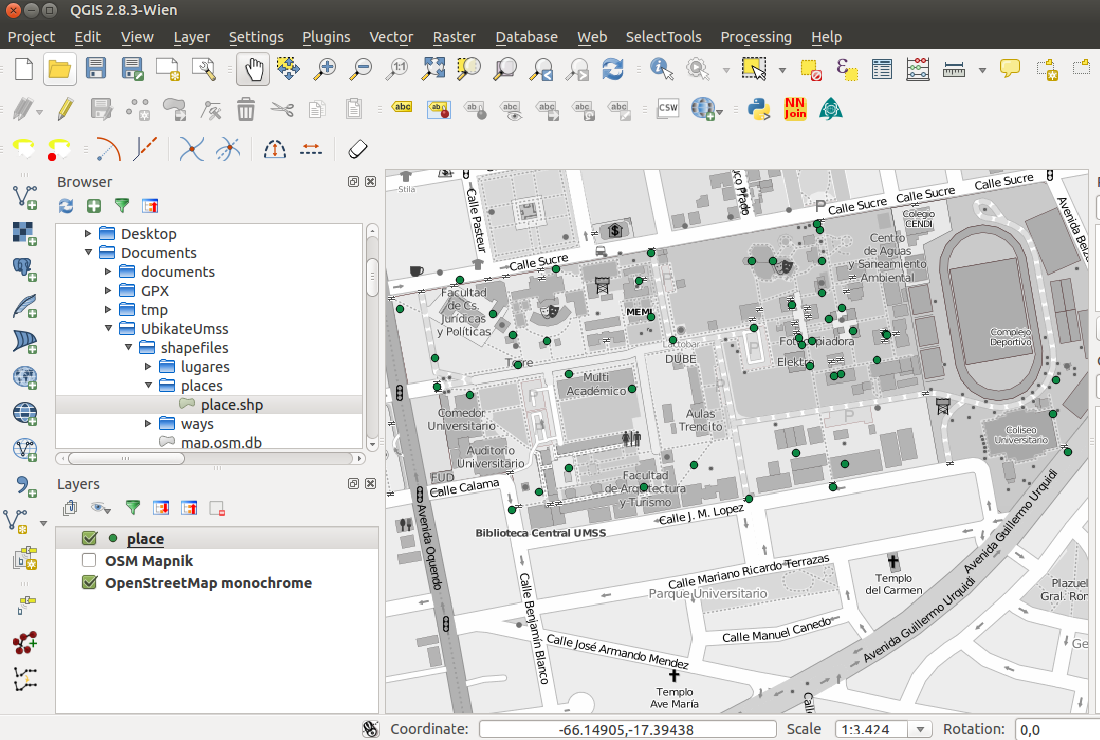
\includegraphics[width=1\textwidth]{qgis_places}
    \caption*{Fuente: Elaboración propia}
  \end{center}
\end{figure}

\subsubsection{RF002}
\label{subs:RF002}

Para poder determinar una base de datos se investigó las diferentes opciones disponibles que tenga la capacidad de manejar información geoespacial y tras la investigación que se puede apreciar en \ref{sec:base_de_datos}, se instaló PostgreSQL 9.4.8 sobre Linux Ubuntu 15.10, y para manejar datos geoespaciales se necesitó instalar PostGIS 2.1.8, para poder acceder a las librerías necesarias para almacenar datos geo-referenciados.\\

El resultado de esta tarea se puede apreciar en el manual de instalación.\\

\subsubsection{RF003}
\label{subs:RF003}

Para esta tarea se hizo uso de una herramienta disponible para postgres, \emph{shp2pgsql}, que permite la conversion de un archivo shapefile a un archivo sql.

\begin{verbatim}
  $ shp2pgsql -s 4326 -I -S -c -d ~/Documents/places.shp > places.sql
\end{verbatim}

Con el anterior comando se tiene como resultado un archivo .sql, el cual es ingresado en la base de datos ya configurada, de esta forma nuestra base de datos ya contiene una tabla geoespacial con datos de tipo POINT, los cuales representan los lugares dentro del campus de la UMSS.\\

El archivo sql resultante es cargado a la base de datos con el siguiente comando.\\

\begin{verbatim}
  $ psql -d db_ubikate -U db_admin -f /Documents/places.sql
\end{verbatim}

\begin{figure}[H]
  \begin{center}
    \caption{Herramienta grafica de PostgreSQL (pgAdmin) con la tabla de Lugares desplegada.}
    \label{fig:postgres_places}
    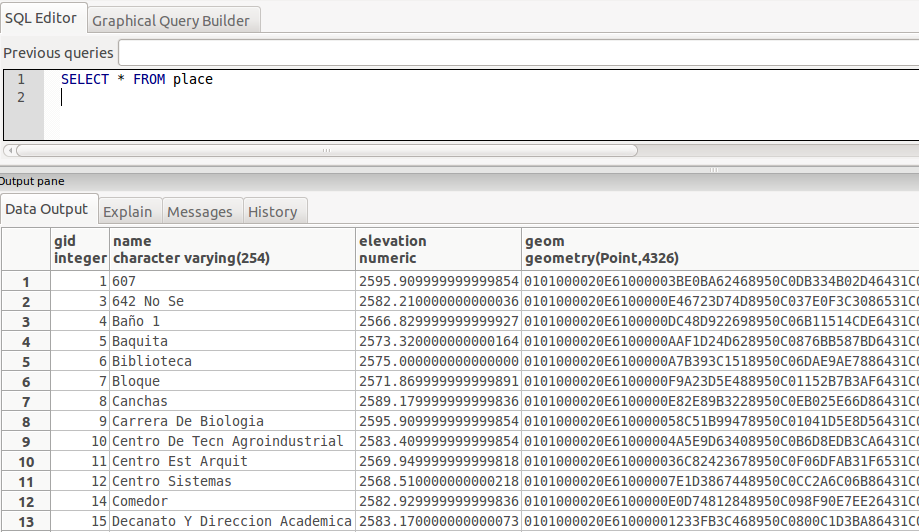
\includegraphics[width=1\textwidth]{iteration1/postgres_places}
    \caption*{Fuente: Elaboración propia}
  \end{center}
\end{figure}

En la figura \ref{fig:postgres_places} se puede observar que la columna \emph{Elevation} contiene datos que el GPS Garmin Nuvi 1300 genera al momento de guardar un punto, en el presente caso es irrelevante.\\

\subsubsection{RF004}
\label{subs:RF004}

Para completar esta tarea se procedió a instalar y configurar el framework de desarrollo Ember JS, que nos ayudará en la implementación del frontend de la aplicación o la capa que interactúa con el usuaria, y Express JS, el cual manejara el backend de la aplicación, básicamente se encarga de la lógica del sistema y la comunicación con la base de datos.\\

\begin{figure}[H]
  \begin{center}
    \caption{Vista de la lista de Lugares registrados en el sistema.}
    \label{fig:places_index}
    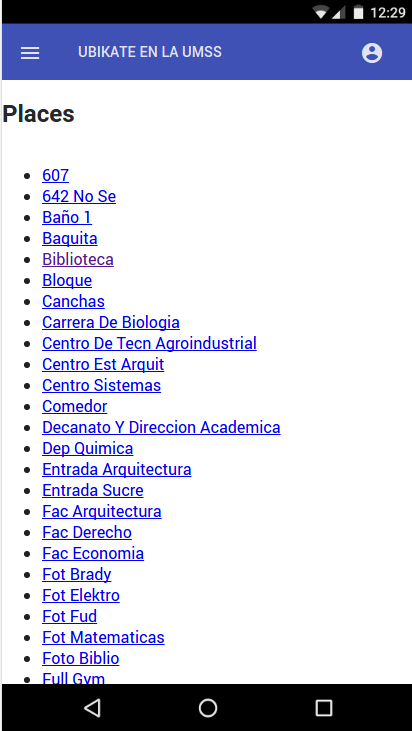
\includegraphics[width=0.5\textwidth]{iteration1/places_index}
    \caption*{Fuente: Elaboración propia}
  \end{center}
\end{figure}

\subsubsection{RF005}
\label{subs:RF005}

\begin{figure}[H]
  \begin{center}
    \caption{Vista de la búsqueda de lugares a través de un cajón de búsqueda.}
    \label{fig:places_search}
    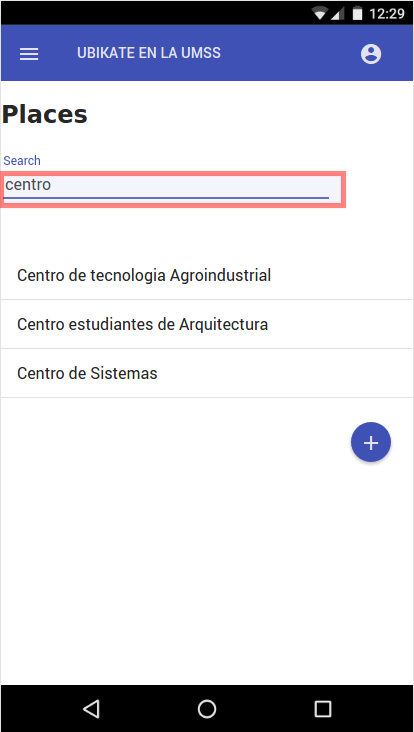
\includegraphics[width=0.5\textwidth]{iteration1/places_search}
    \caption*{Fuente: Elaboración propia}
  \end{center}
\end{figure}


\subsubsection{RF006}
\label{subs:RF006}

Para implementar esta funcionalidad del sistema fue necesario utilizar las funcionalidad de Ember JS.

\begin{verbatim}
  {{#paper-item class="md-1-line" onClick=(transition-to 'places.show' place)}}
      <div class="md-list-item-text">
          <span>{{place.name}}</span>
      </div>
  {{/paper-item}}
\end{verbatim}

\subsubsection{RF007}
\label{subs:RF007}



\begin{figure}[H]
  \begin{center}
    \caption{Vista de la Información de un Lugar.}
    \label{fig:place_show}
    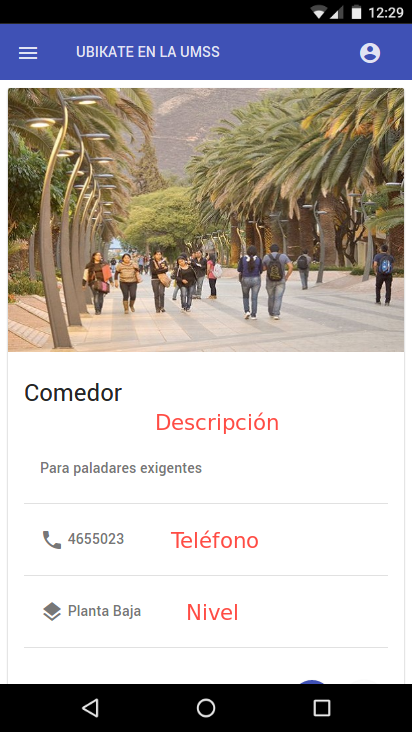
\includegraphics[width=0.5\textwidth]{iteration1/place_show}
    \caption*{Fuente: Elaboración propia}
  \end{center}
\end{figure}


\subsubsection{RF008}
\label{subs:RF008}
% RF008: El usuario puede ver el teléfono del lugar

\subsubsection{RF009}
\label{subs:RF009}
% RF009: El usuario puede ver en qué piso se encuentra el lugar

\subsubsection{RF010}
\label{subs:RF010}
 % RF010: El usuario puede ver una imagen del lugar
 El hecho de visualizar las imagenes dentro de la aplicacion se tiene q pensar en donde se van a guardar las imagenes
 Para realizar esta tarea se hizo uso de Cloudinary

\subsubsection{TS001}
\label{subs:TS001}

Pruebas funcionales


\subsubsection{TS002}
\label{subs:TS002}

Pruebas funcionales

\subsection{Registrar el Avance}
\label{sub:iteracion1_avance}

\subsection{Verificación}
\label{sub:iteracion1_verificacion}
